\subsection{A priori error estimates}

The need for \textit{h-adaptivity} arises from the inefficiency encountered solving the Poisson problem over sequences of uniform meshes while working with pathological exact solutions such as \eqref{pathological_square} and \eqref{pathological_lshape}.

The first step to implement \textit{h-adaptivity} is to evaluate the $\LT$ error on each element and then refine the element with the highest error according to a specific refinement strategy.

The strategy of choice can be outlined as follows:

\begin{enumerate}
    \item For polygons with $N_e \leq 4$, the refiner adds a single node at the polygon's centroid and then connects each edge's midpoint to this new node, creating $N_e$ new quadrilaterals.
    \item For polygons with $N_e > 4$, the refiner adds $N_e$ new nodes at the midpoints of the segments connecting the polygon's centroid to the midpoints of its edges. The refiner then connects these points to form quadrilaterals along the polygon's edges and creates a new smaller polygon by connecting all the new internal nodes.
\end{enumerate}

Refinement occurs by setting a refinement percentage and marking all elements where the local error exceeds that percentage of the highest error.

Error trends and refined meshes in the following pages.

\newpage
\subsubsection{Errors}

\begin{figure}[!ht]
	\centering
	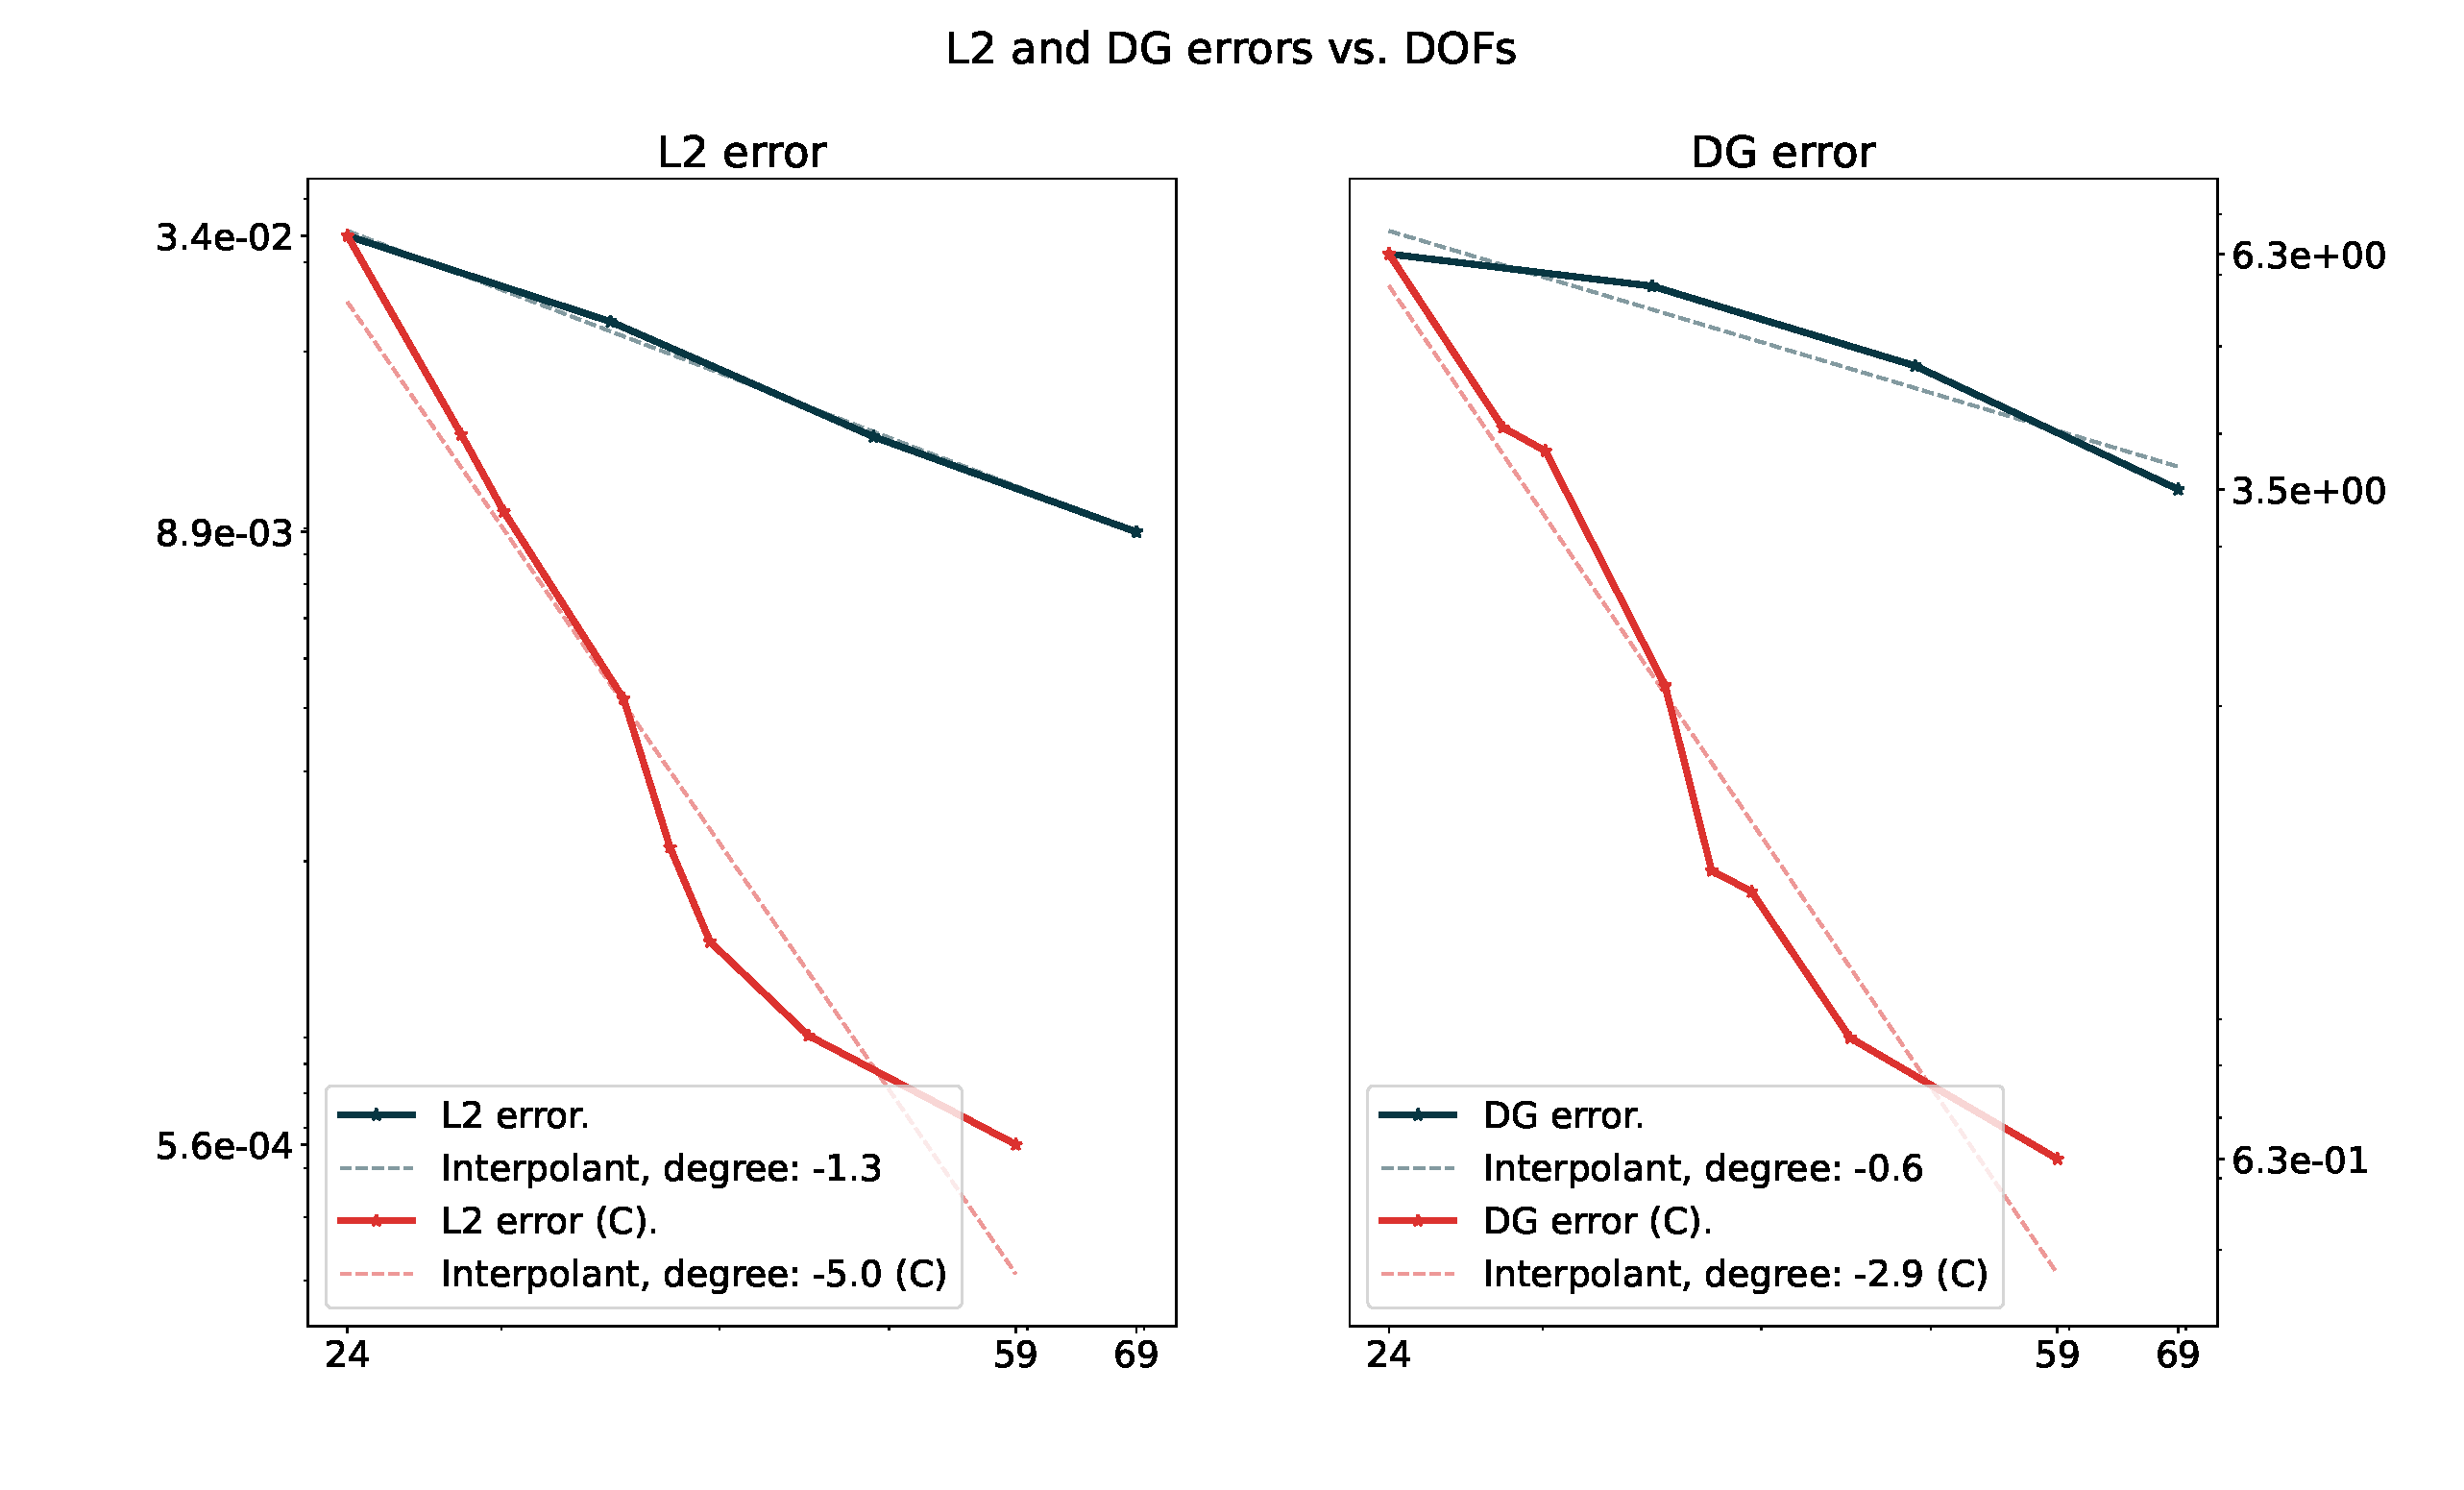
\includegraphics[trim=0cm 0.5cm 0cm 2cm, clip, width=16cm]{square_h.pdf}
    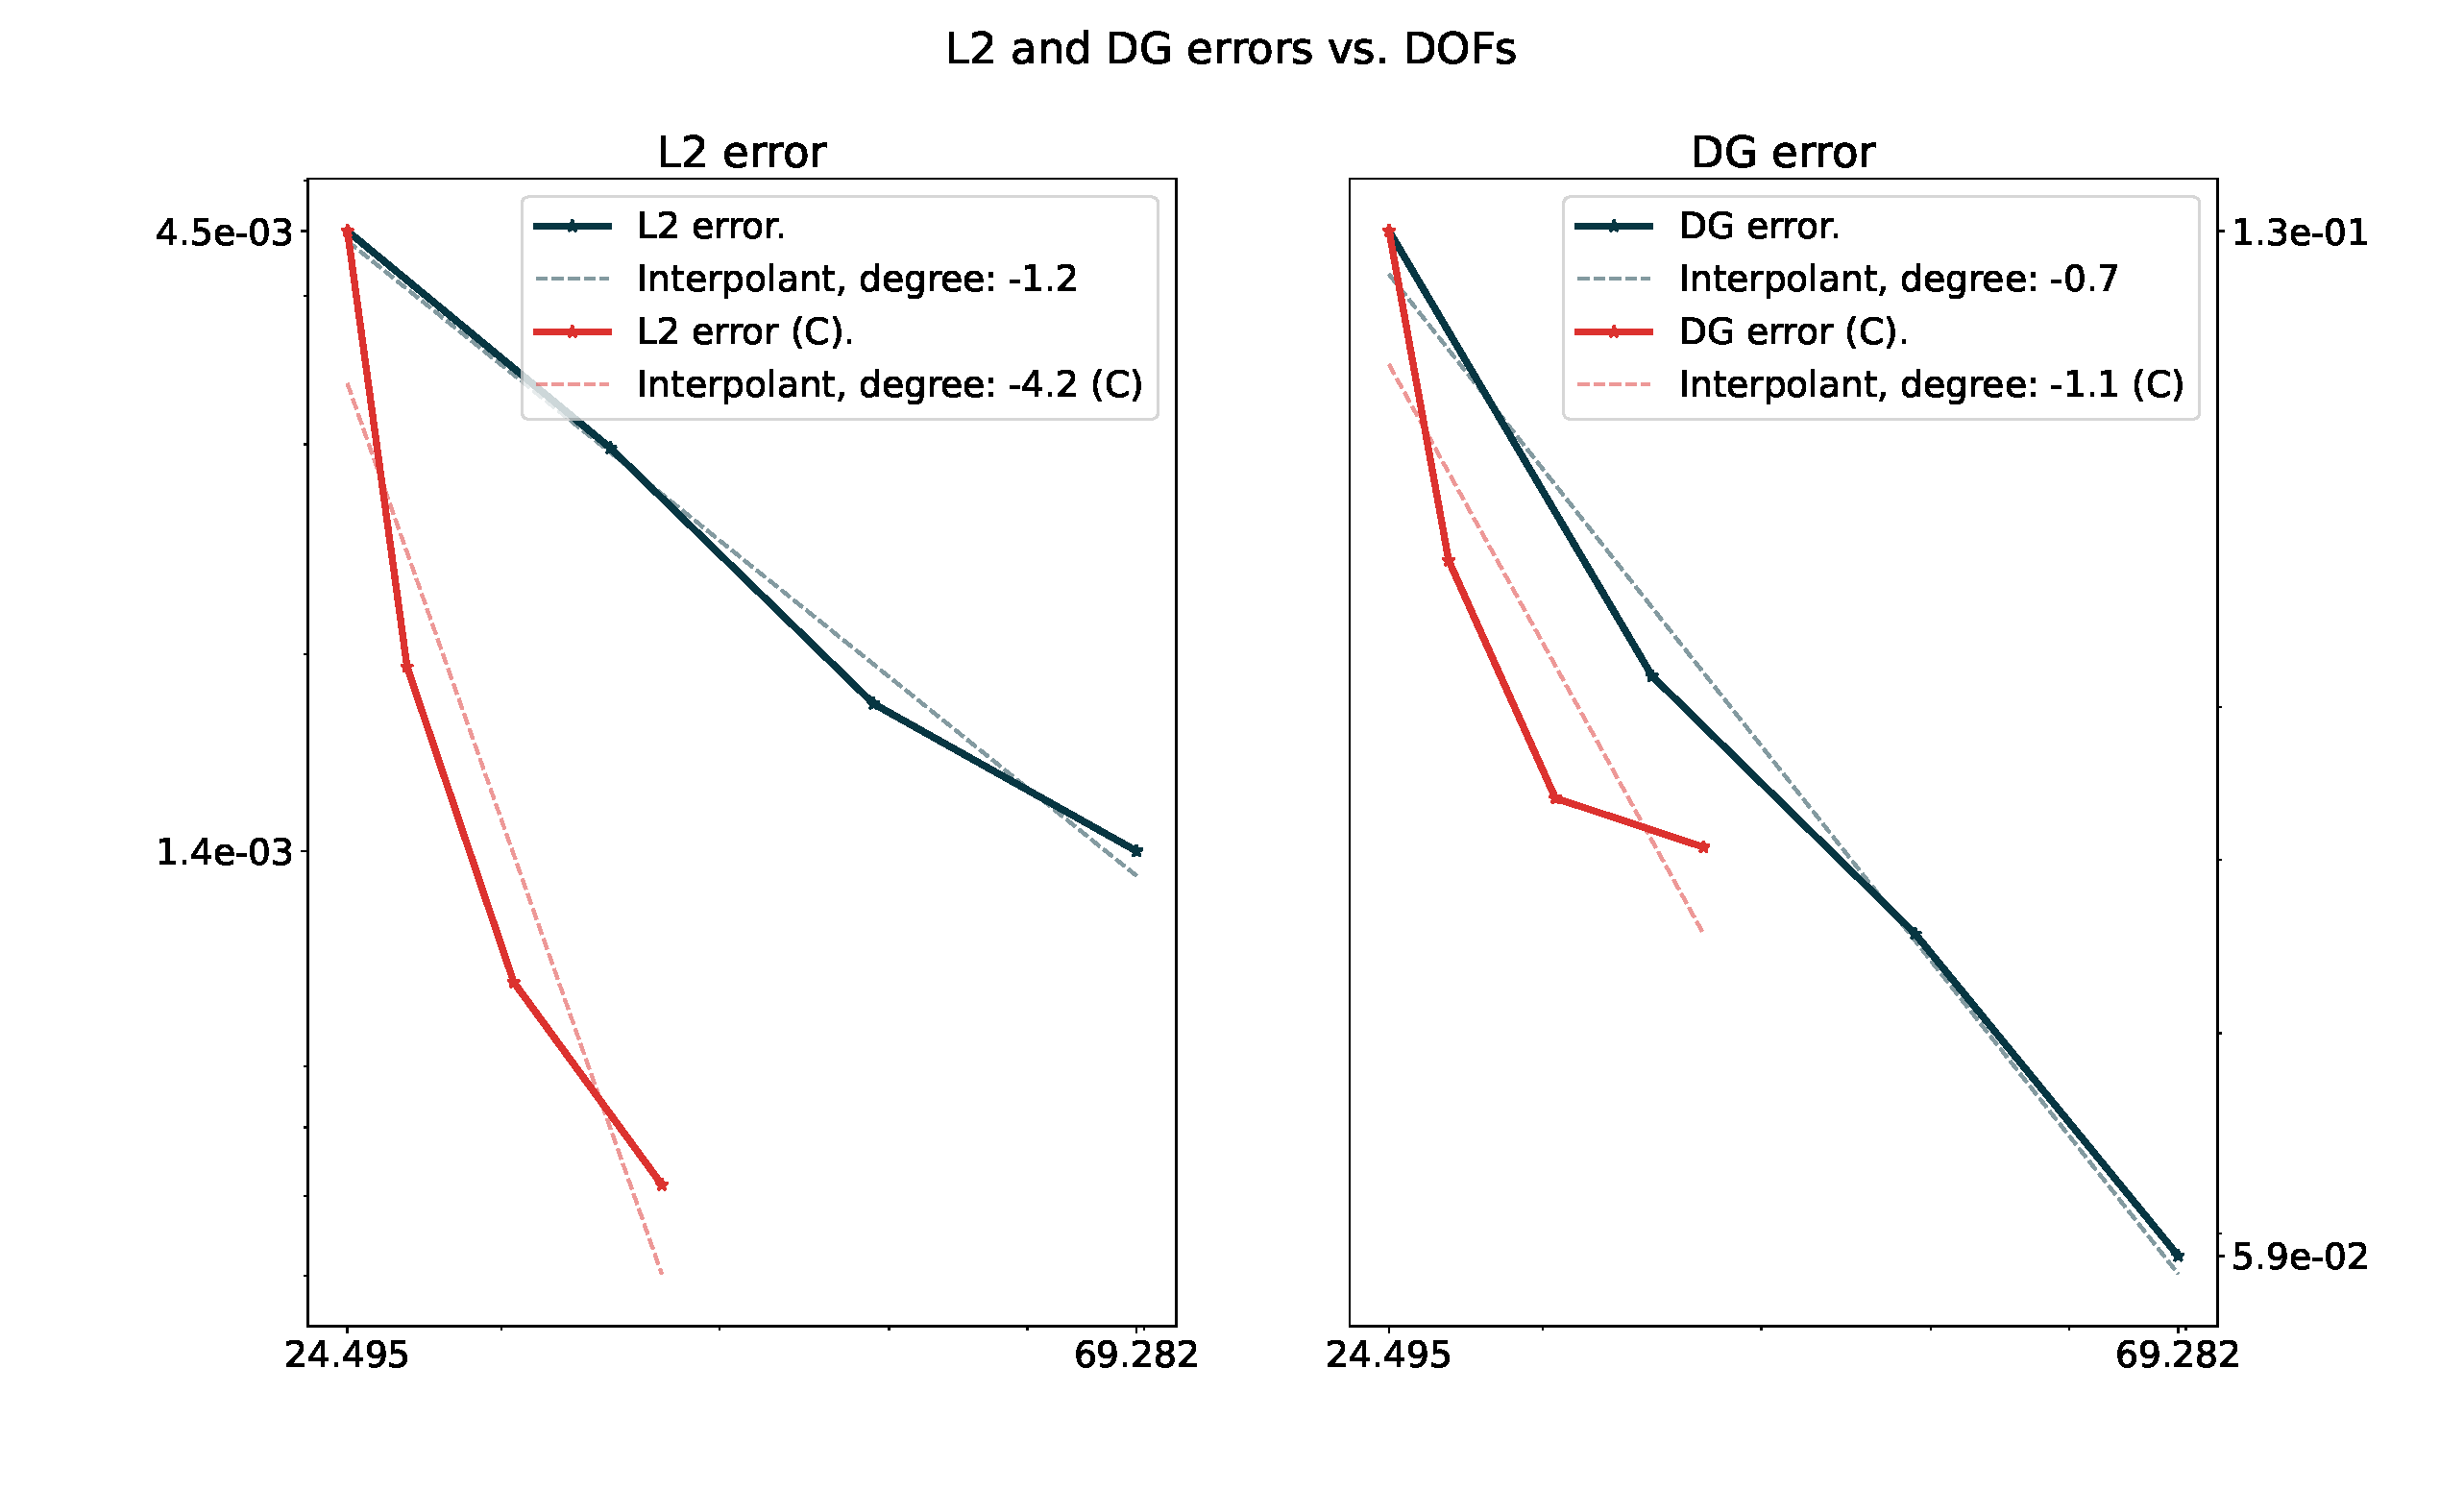
\includegraphics[trim=0cm 0.5cm 0cm 2cm, clip, width=16cm]{lshape_h.pdf}
	\caption{Comparison of $\LT$ and DG errors versus $\text{DOFs}^{1/2}$ between a sequence of uniform meshes and \textit{h-adaptively} refined meshes over a square domain (top) and an L-shaped domain (bottom), $k = 2$ and $N \in \{100, 200, 400, 800\}$.}
\end{figure}

\newpage
\subsubsection{Meshes}

\begin{figure}[!ht]
	\centering
	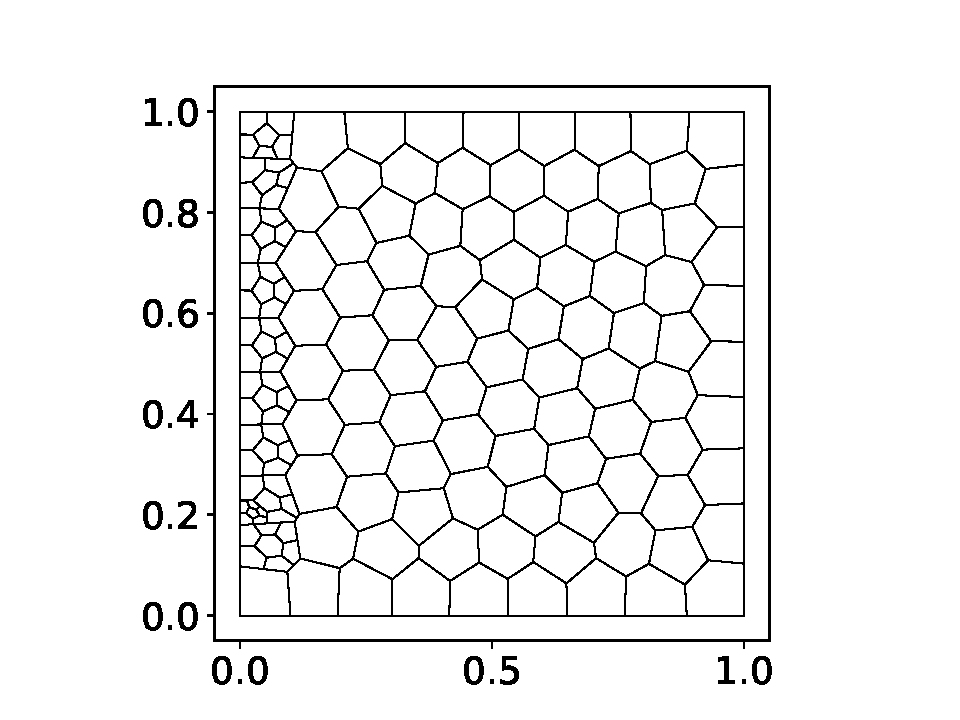
\includegraphics[trim=0cm 0.5cm 0cm 0.5cm, clip, width=5.5cm]{square_100_h0.pdf}
    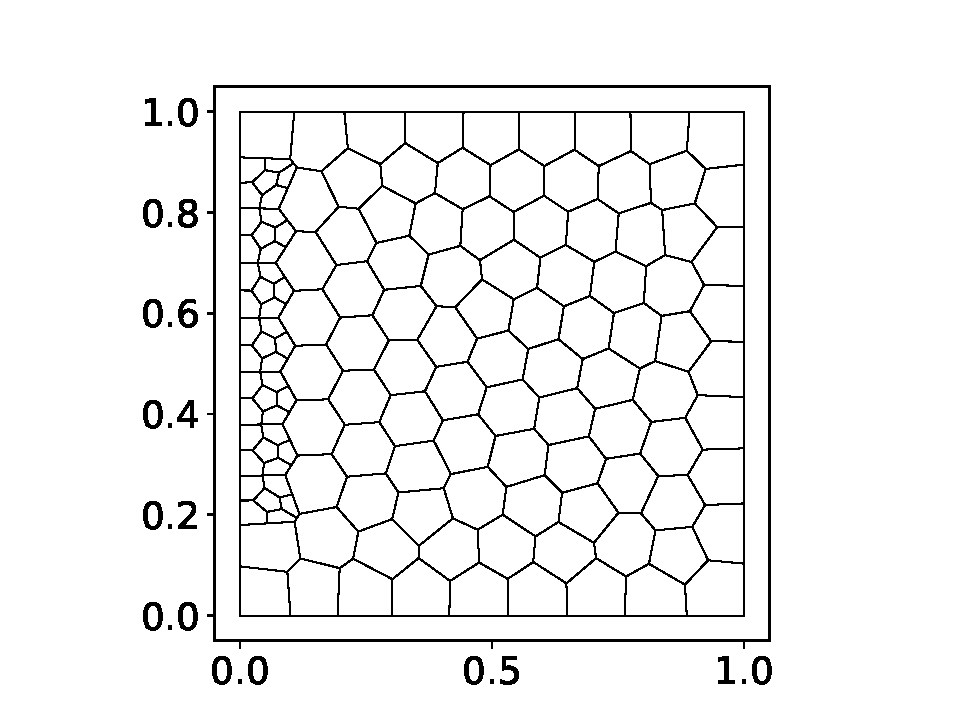
\includegraphics[trim=0cm 0.5cm 0cm 0.5cm, clip, width=5.5cm]{square_100_h1.pdf}
    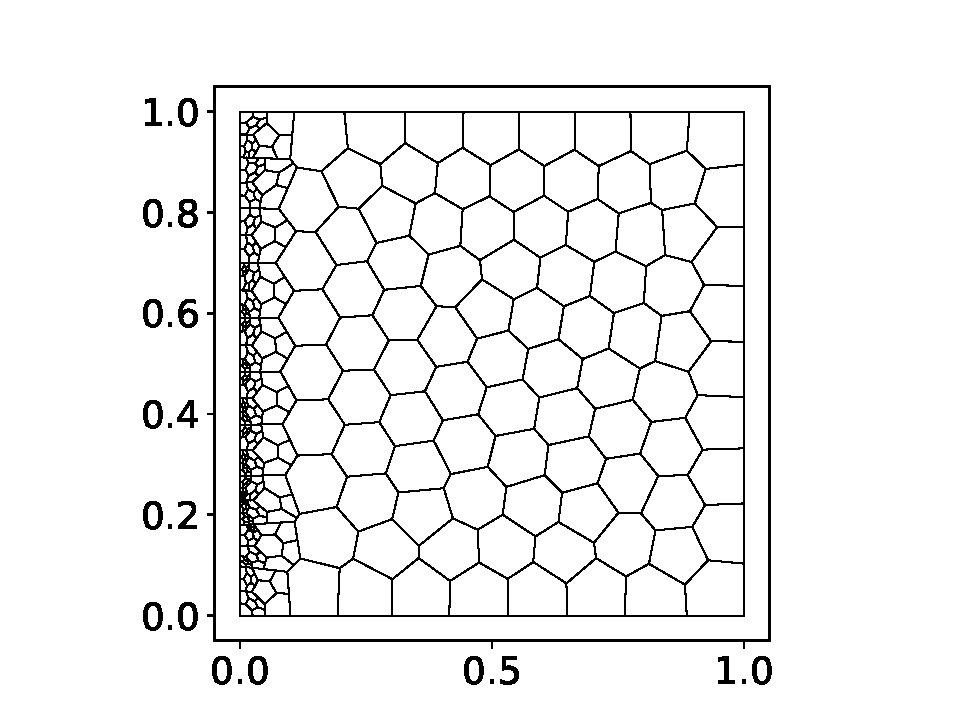
\includegraphics[trim=0cm 0.5cm 0cm 0.5cm, clip, width=5.5cm]{square_100_h2.pdf}
	\caption{Square mesh after 2, 4 and 6 refinements, $N_0 = 100$.}
\end{figure}

\begin{figure}[!ht]
	\centering
	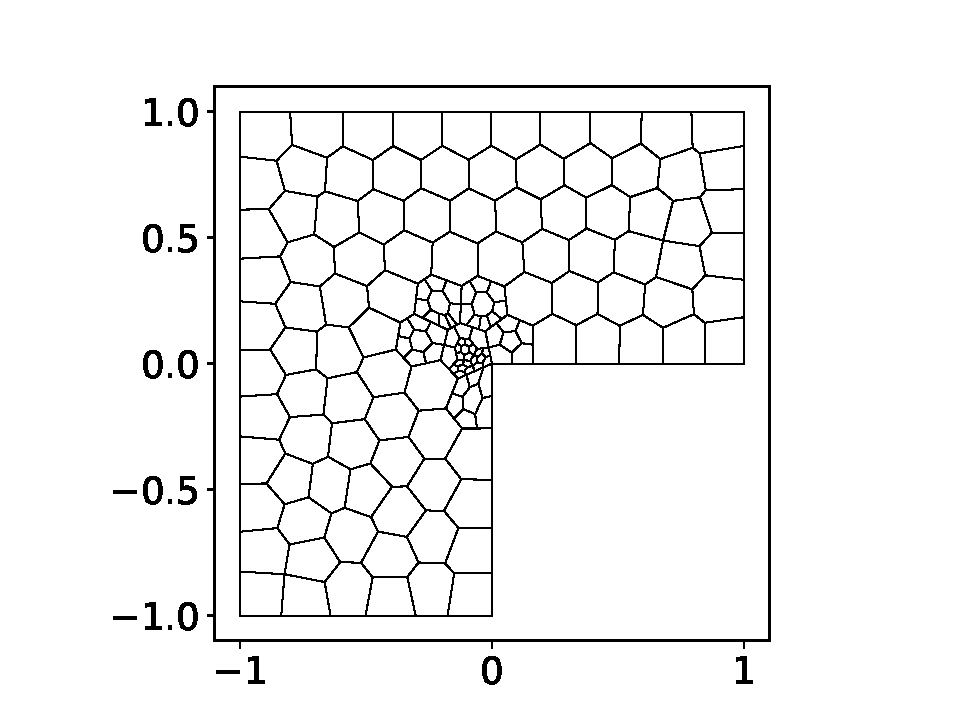
\includegraphics[trim=0cm 0.5cm 0cm 0.5cm, clip, width=5.5cm]{lshape_100_h0.pdf}
    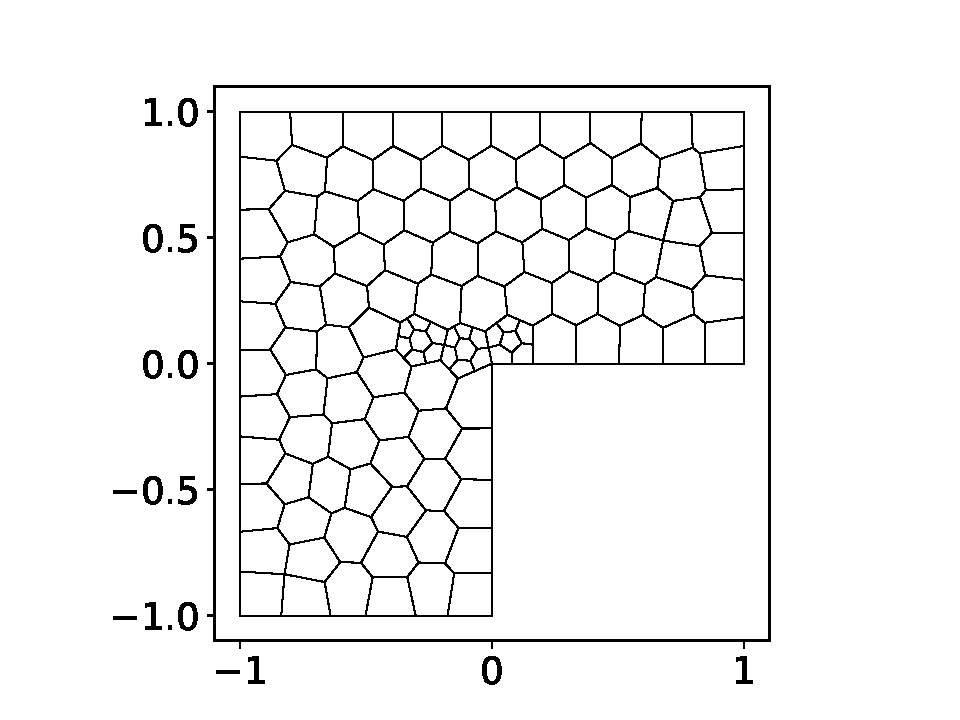
\includegraphics[trim=0cm 0.5cm 0cm 0.5cm, clip, width=5.5cm]{lshape_100_h1.pdf}
    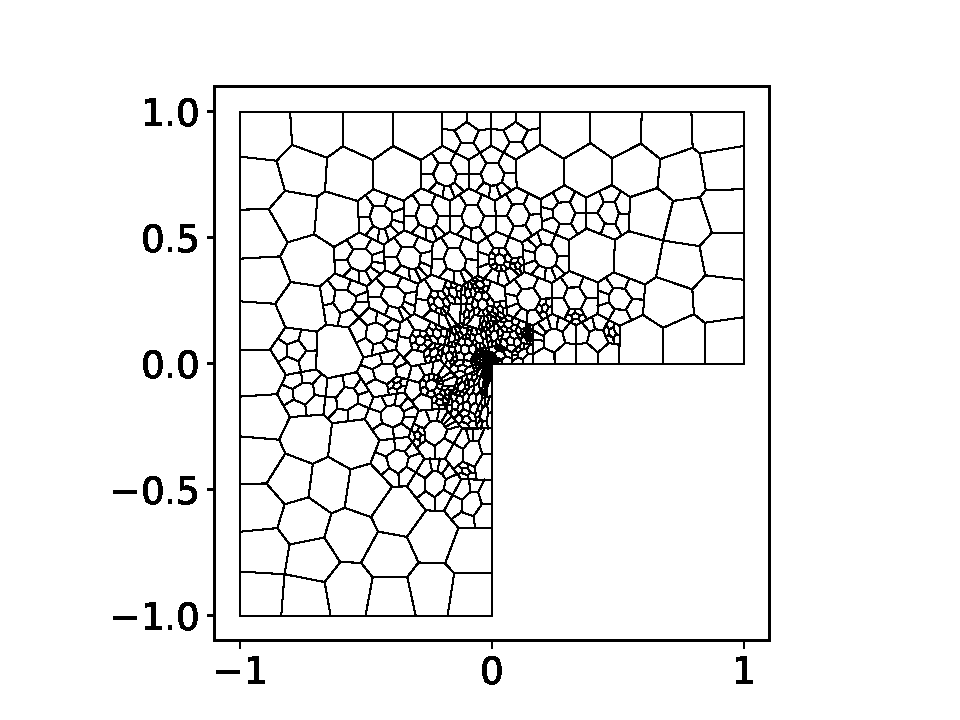
\includegraphics[trim=0cm 0.5cm 0cm 0.5cm, clip, width=5.5cm]{lshape_100_h2.pdf}
	\caption{L-shaped mesh after 2, 4 and 6 refinements, $N_0 = 100$.}
\end{figure}

\newpage
\subsection{A posteriori error estimates}

The second step to implement \textit{h-adaptivity} is to define an \textit{a posteriori} error estimator, enabling the identification of elements that need refinement without requiring any information about the exact solution.

\cite{Cangiani2023} One possible approach considers the following upper bound on the error:

\begin{gather}
	\lVert u - u^k_h \rVert_{\LT(\Omega)} \leq C_{ub} \sum_{K \in \Tau_h} (R_K^2 + O_K^2),
\end{gather}

where:

\begin{gather}
	R_K^2 = R_{K, E}^2 + R_{K, N}^2 + R_{K, J}^2 + R_{K, T}^2
\end{gather}

is the local estimator and:

\begin{gather}
	O_K^2 = O_{K, E}^2 + O_{K, J}^2 + O_{K, T}^2
\end{gather}

is the local data oscillation, with each term given by:

\begin{align}
	R_{K, E} &= \lVert h (\bar{f} + \Delta u^k_h) \rVert_{\LT(K)}, \\
	R_{K, N} &= \lVert h^{1/2} \llbracket \grad u^k_h \cdot \Vector{n} \rrbracket \rVert_{\LT(\partial K)}, \\
	R^2_{K, J} &= \lVert \sigma^{1/2} \llbracket u^k_h \rrbracket \rVert^2_{\LT(\partial K \cap \Gamma_{i})} + \lVert \sigma^{1/2} (u^k_h - \bar{g}) \rVert^2_{\LT(\partial K \cap \partial \Omega)}, \\
	R^2_{K, T} &= \lVert h^{1/2} \llbracket \grad u^k_h \cdot \Vector{e} \rrbracket \rVert^2_{\LT(\partial K \cap \Gamma_{i})} + \lVert \sigma^{1/2} \grad (u^k_h - \bar{g}) \cdot \Vector{e} \rVert^2_{\LT(\partial K \cap \partial \Omega)}, \\
	O_{K, E} &= \lVert h (f - \bar{f}) \rVert_{\LT(K)}, \\
	O_{K, J} &= \lVert \sigma^{1/2} (g - \bar{g}) \rVert_{\LT(\partial K \cap \partial \Omega)}, \\
	O_{K, T} &= \lVert h^{1/2} \grad (g - \bar{g}) \cdot \Vector{e} \rVert_{\LT(\partial K \cap \partial \Omega)}.
\end{align}

\newpage
\subsubsection{Errors}

\begin{figure}[!ht]
	\centering
	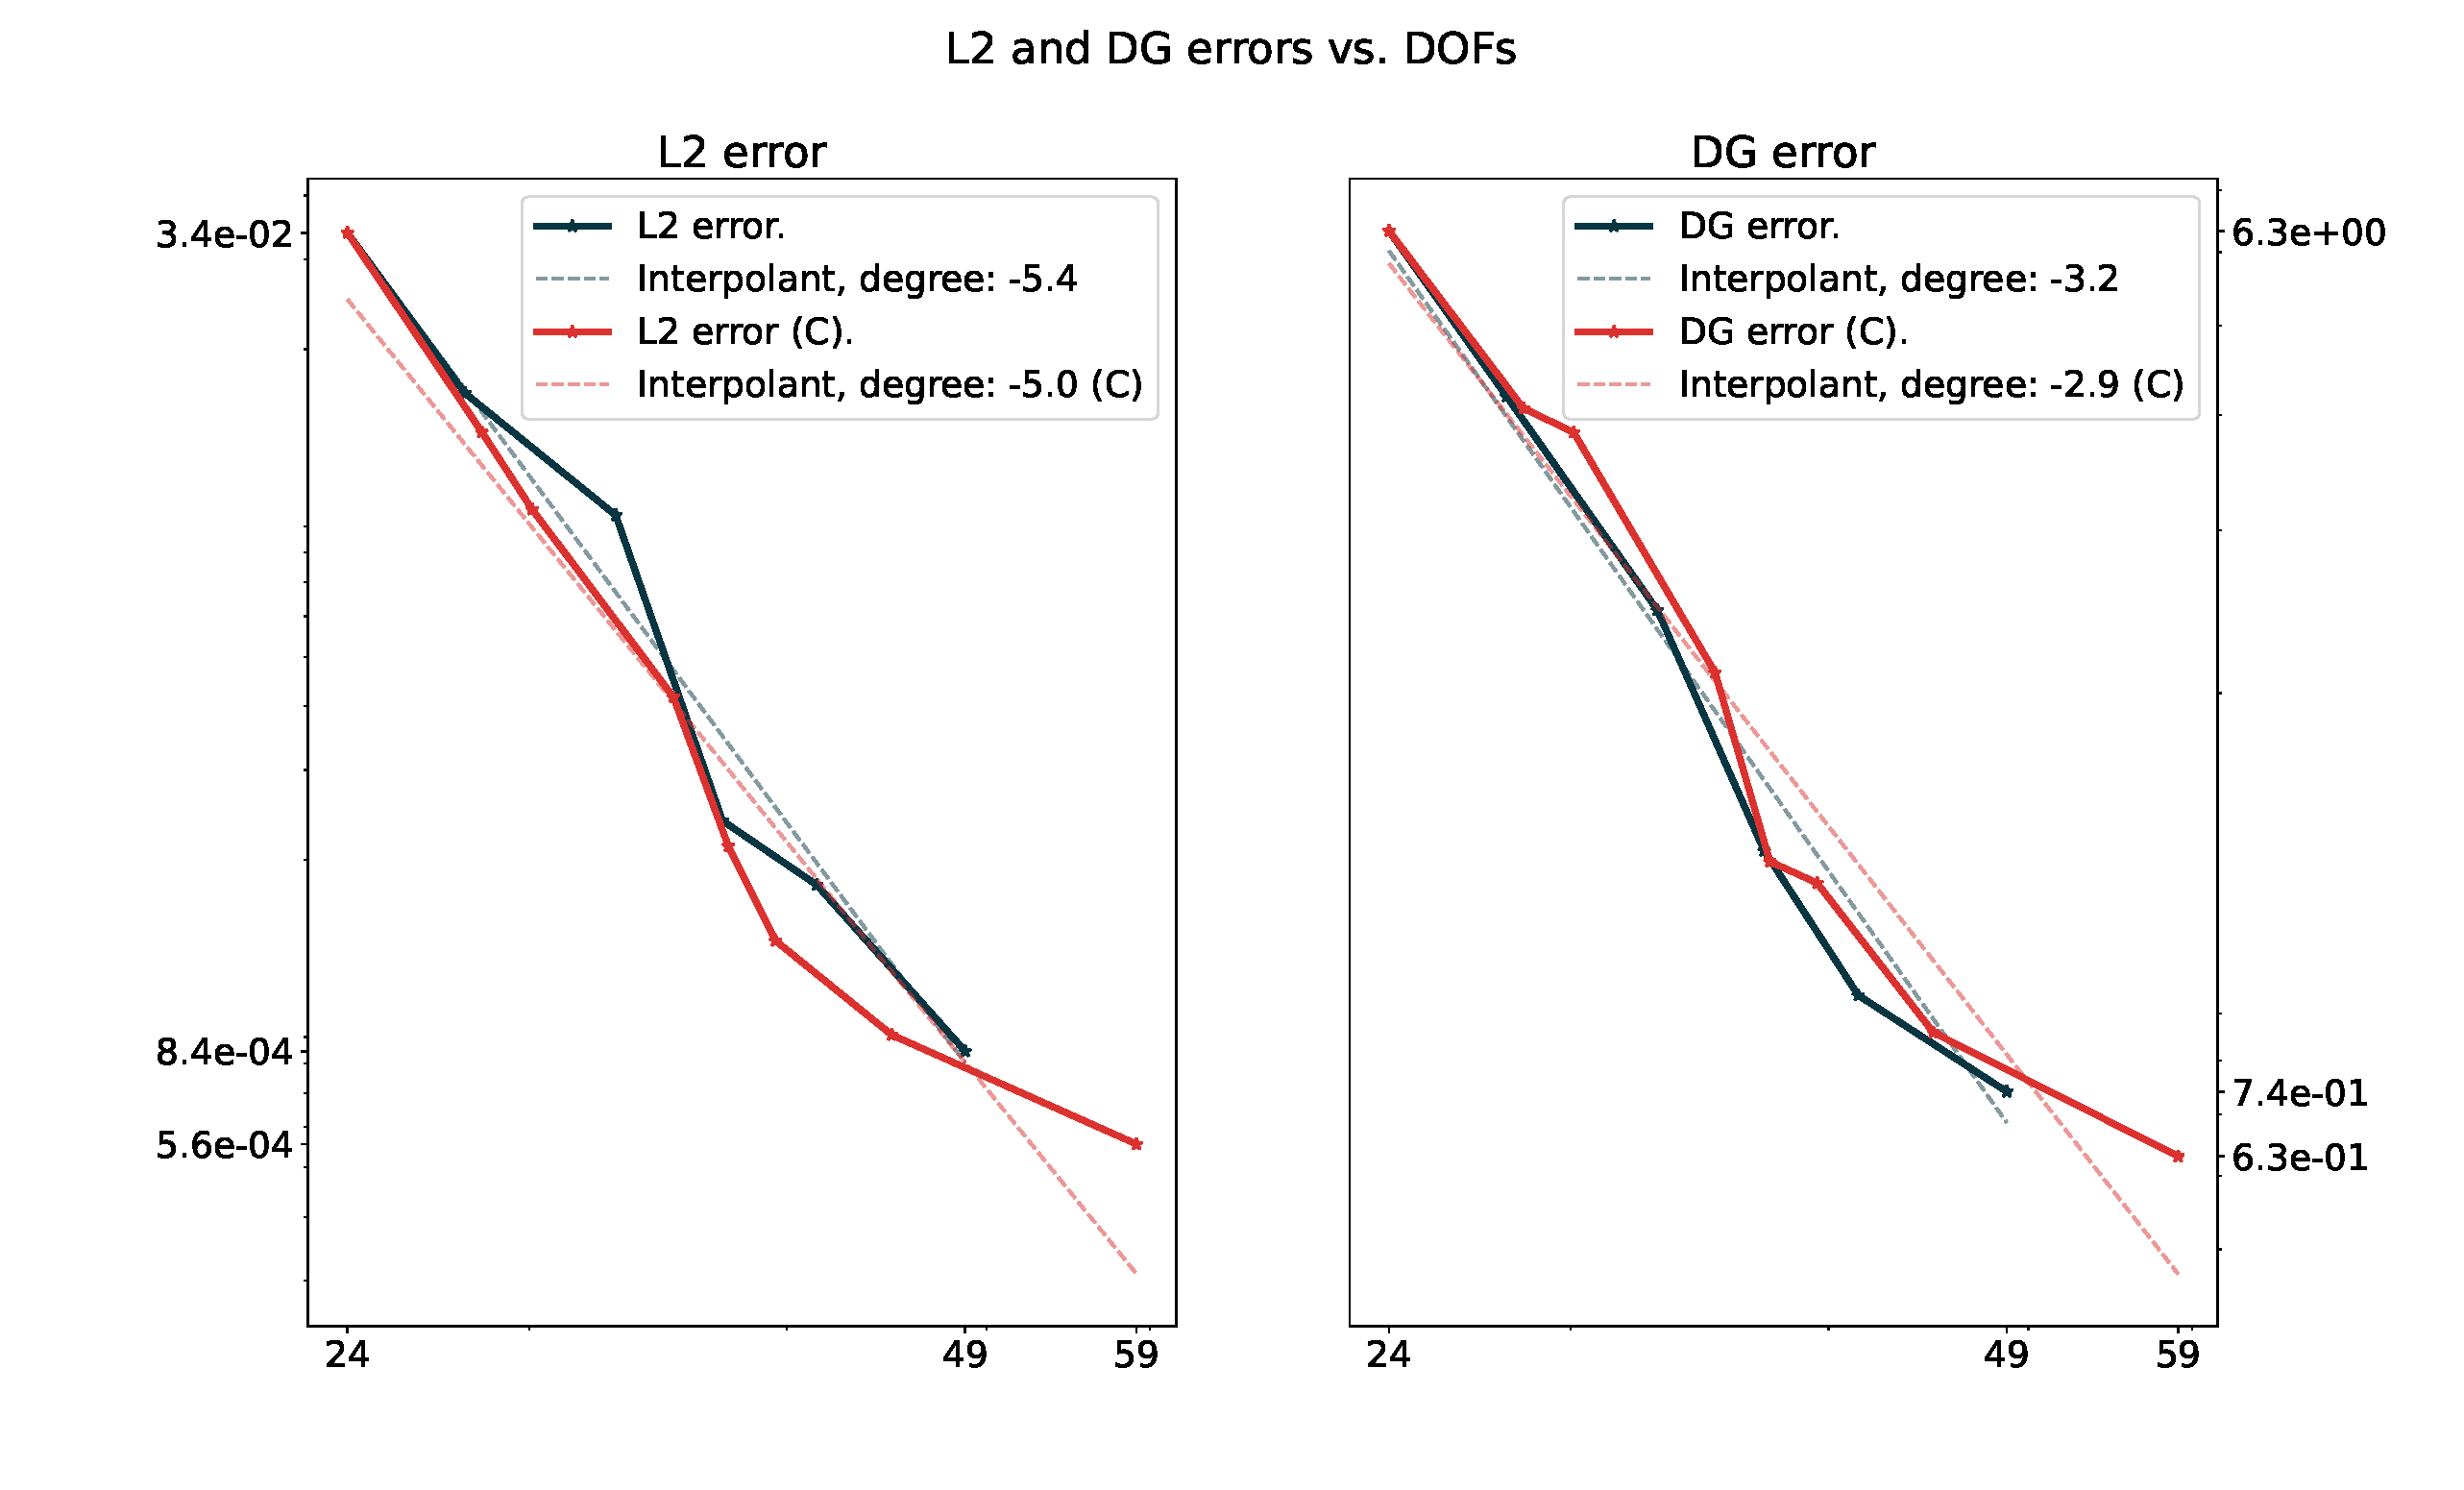
\includegraphics[trim=0cm 0.5cm 0cm 2cm, clip, width=16cm]{square_eh_h.pdf}
    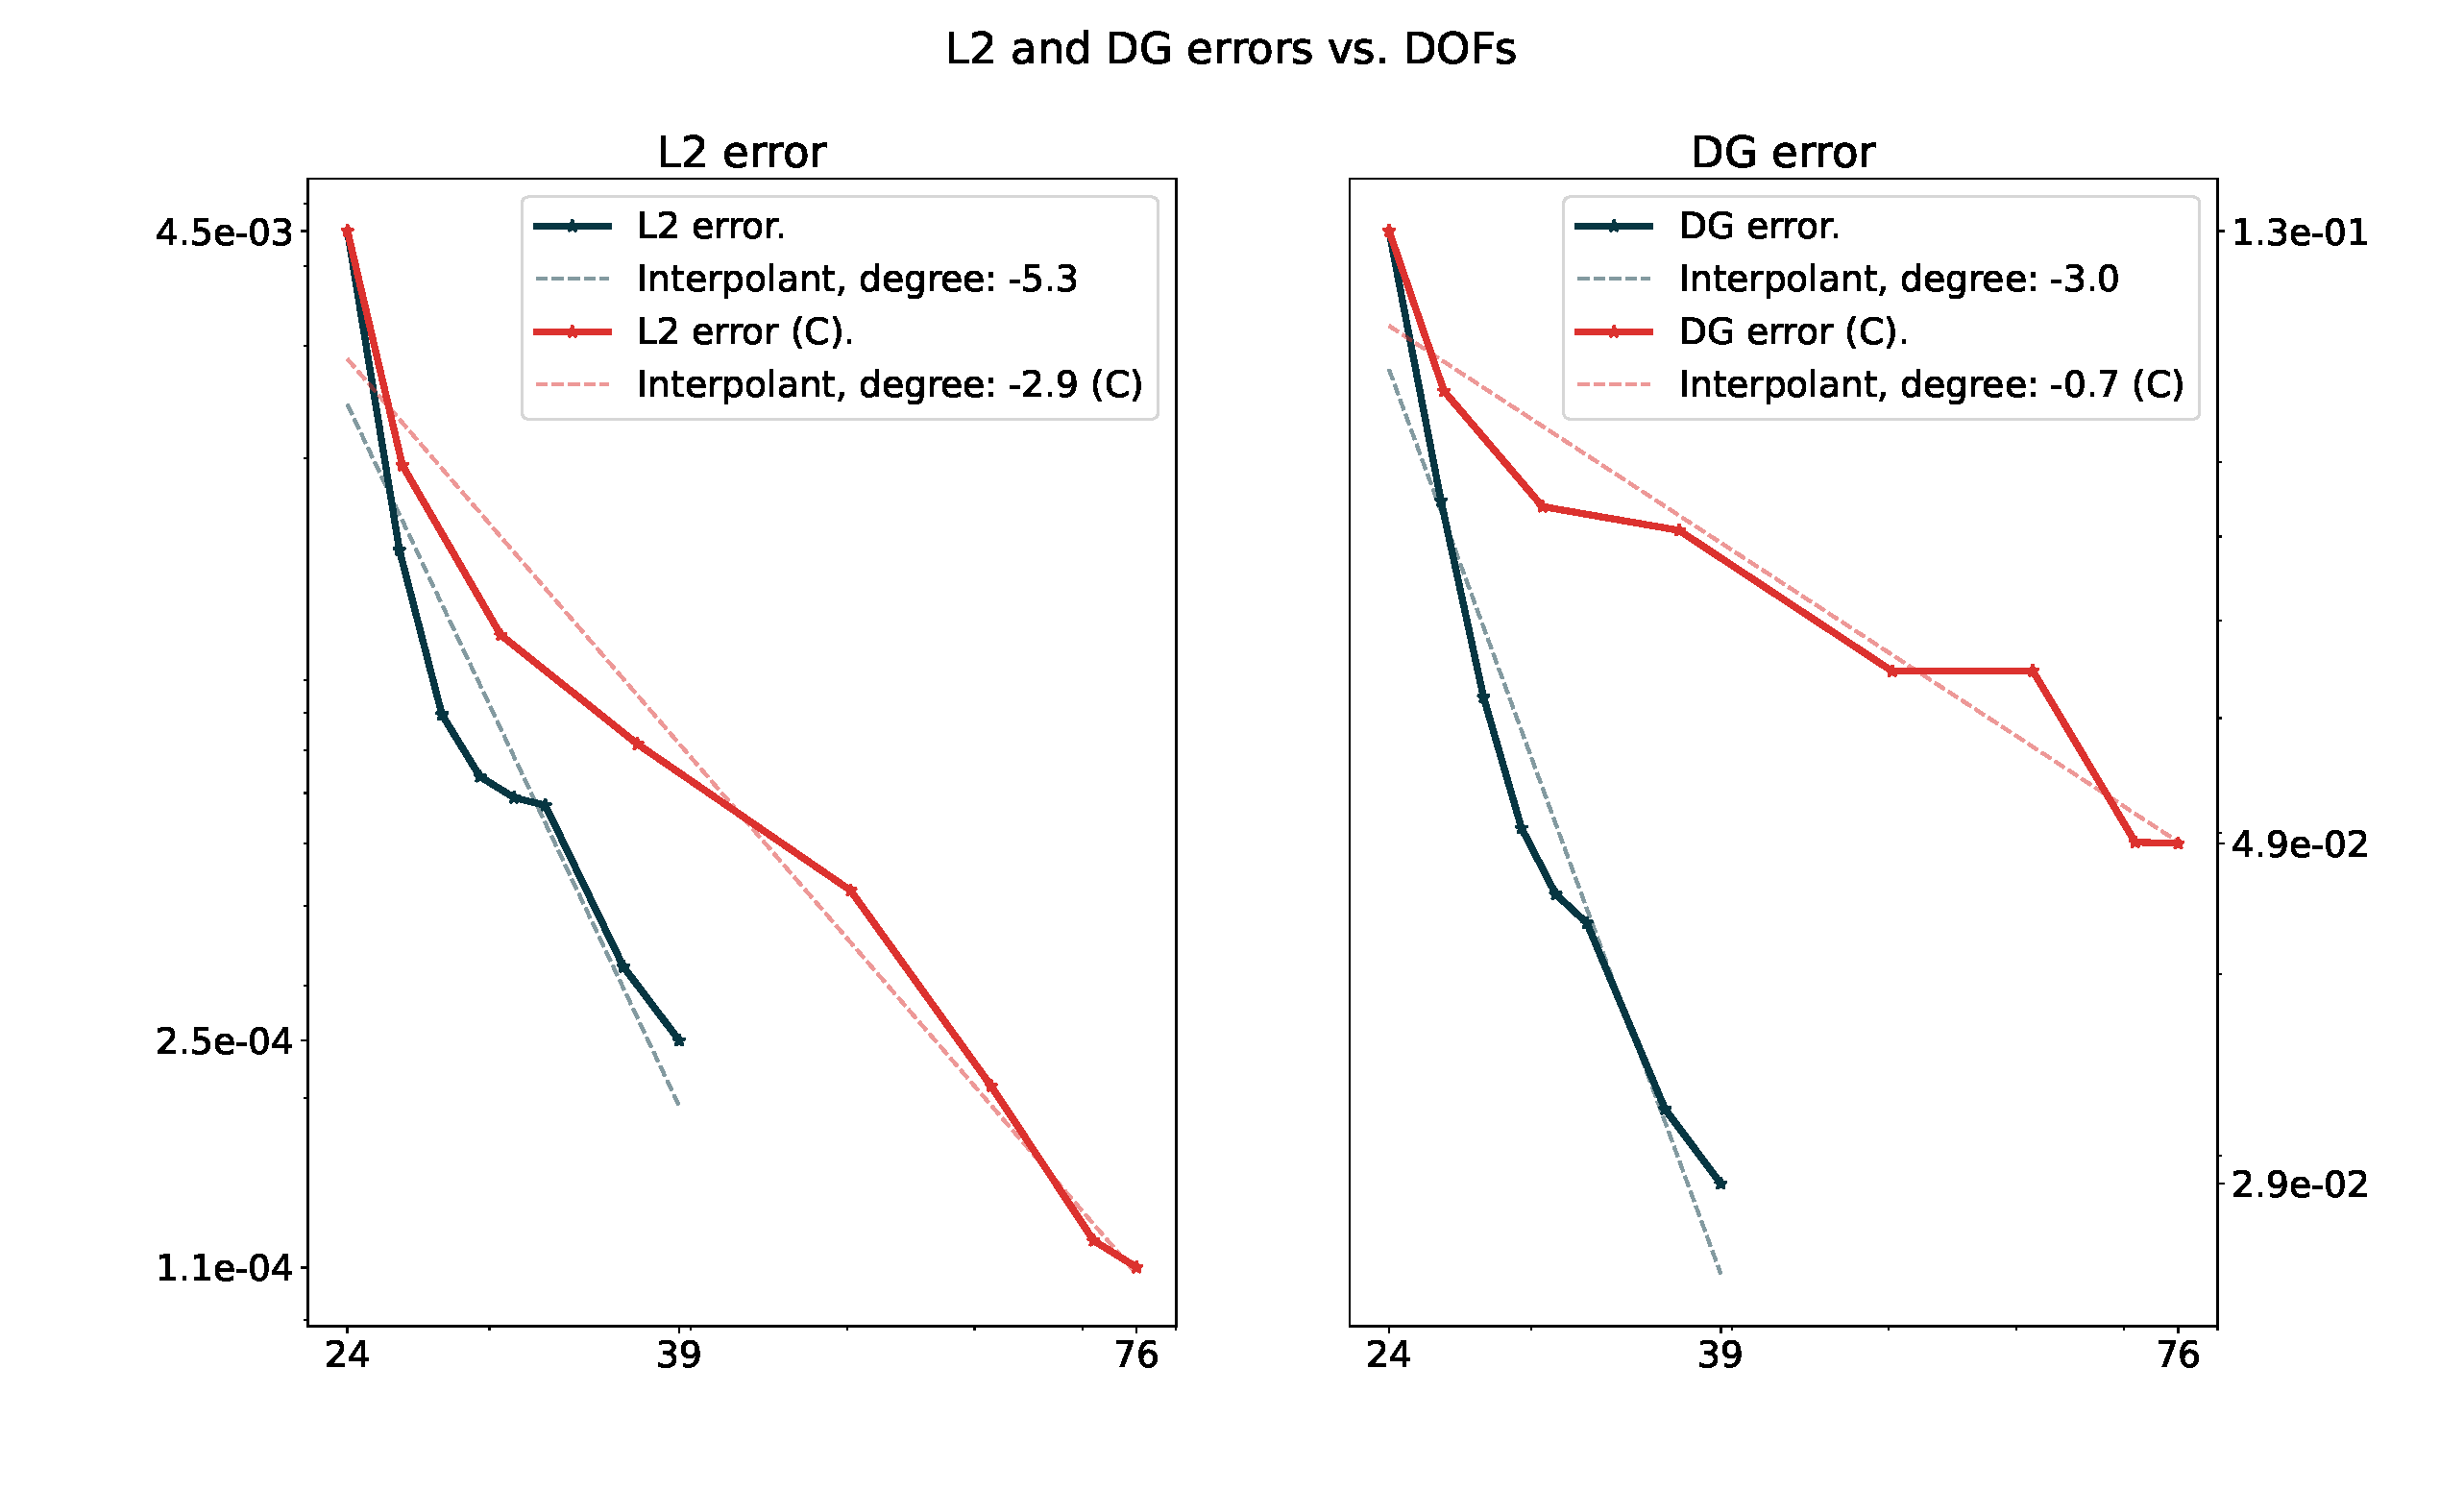
\includegraphics[trim=0cm 0.5cm 0cm 2cm, clip, width=16cm]{lshape_eh_h.pdf}
	\caption{Comparison of $\LT$ and DG errors versus $\text{DOFs}^{1/2}$ between two sequences of \textit{h-adaptively} refined meshes over a square domain (top) and an L-shaped domain (bottom), $k = 2$.}
\end{figure}

\newpage
\subsubsection{Meshes}

\begin{figure}[!ht]
	\centering
	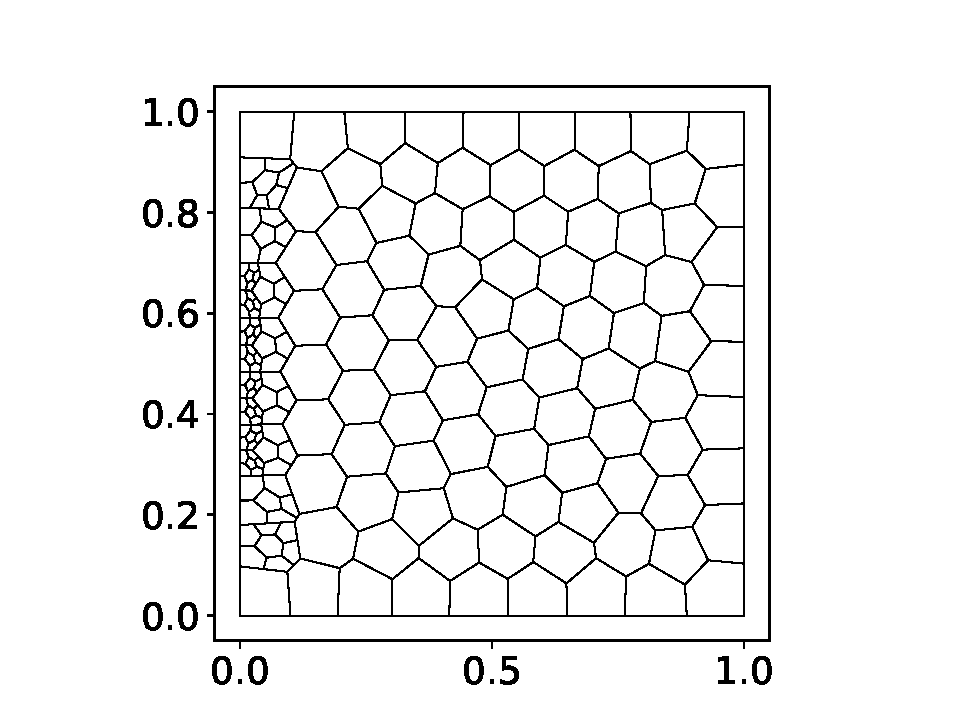
\includegraphics[trim=0cm 0.5cm 0cm 0.5cm, clip, width=5.5cm]{square_100_eh0.pdf}
    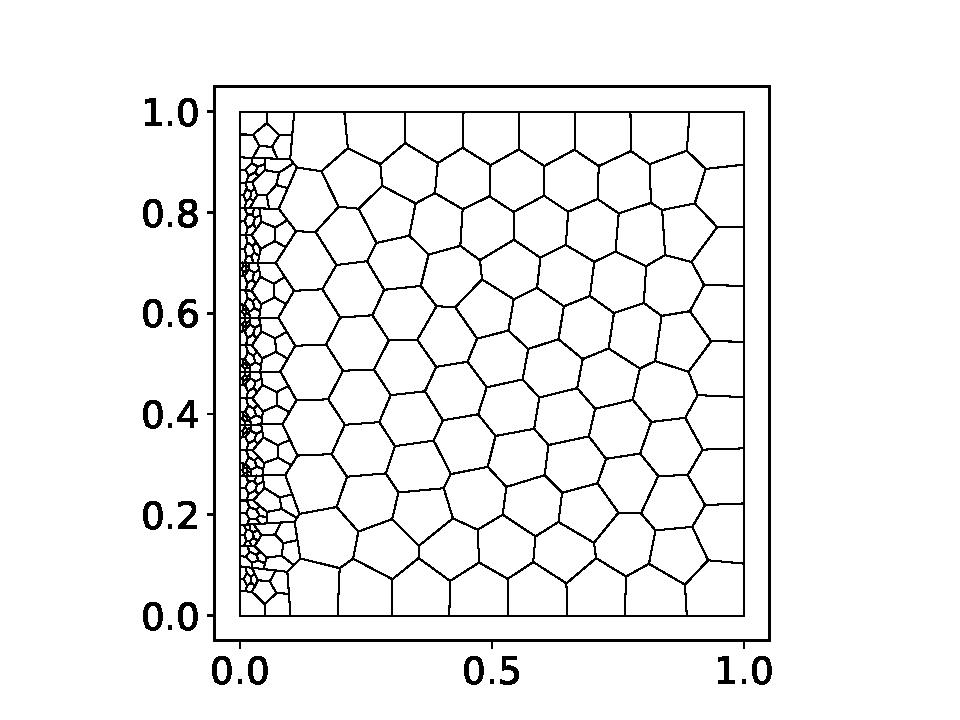
\includegraphics[trim=0cm 0.5cm 0cm 0.5cm, clip, width=5.5cm]{square_100_eh1.pdf}
    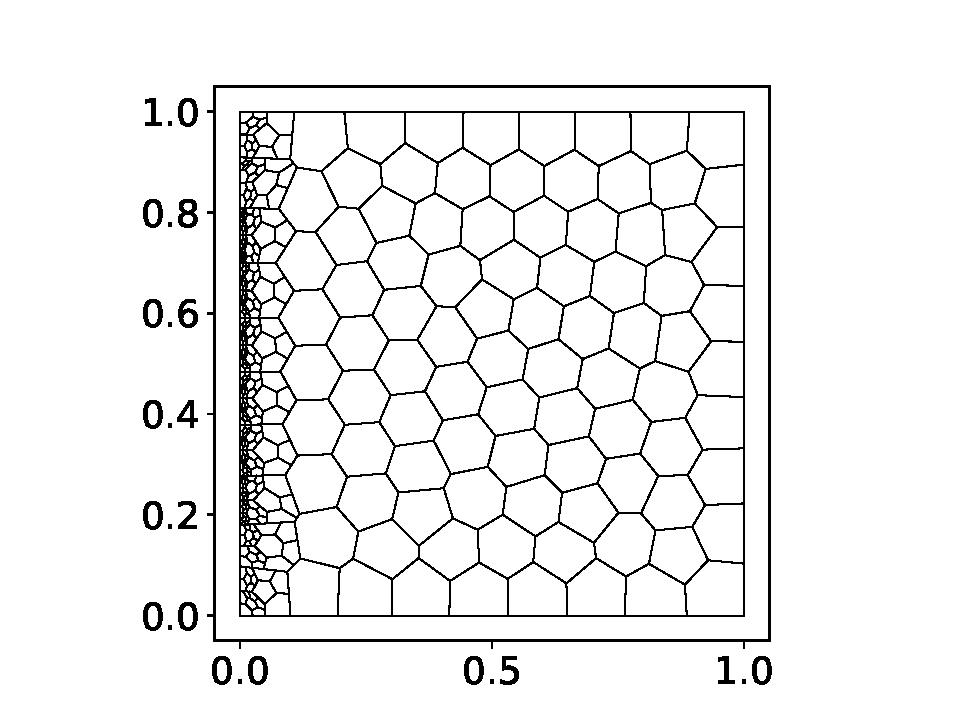
\includegraphics[trim=0cm 0.5cm 0cm 0.5cm, clip, width=5.5cm]{square_100_eh2.pdf}
	\caption{Square mesh after 2, 4 and 6 refinements, $N_0 = 100$.}
\end{figure}

\begin{figure}[!ht]
	\centering
	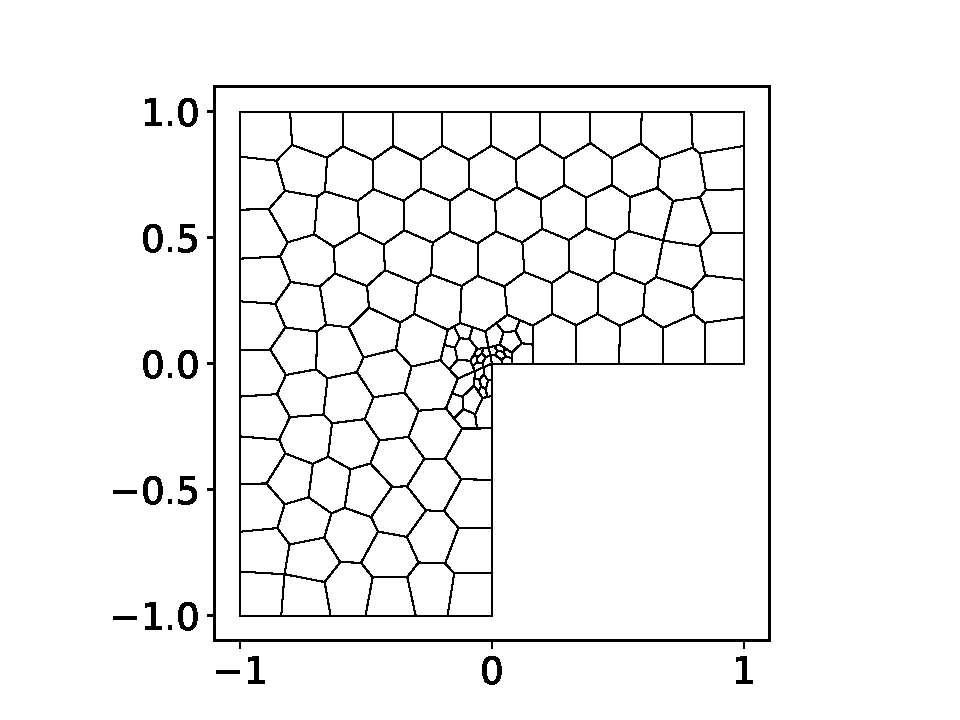
\includegraphics[trim=0cm 0.5cm 0cm 0.5cm, clip, width=5.5cm]{lshape_100_eh0.pdf}
    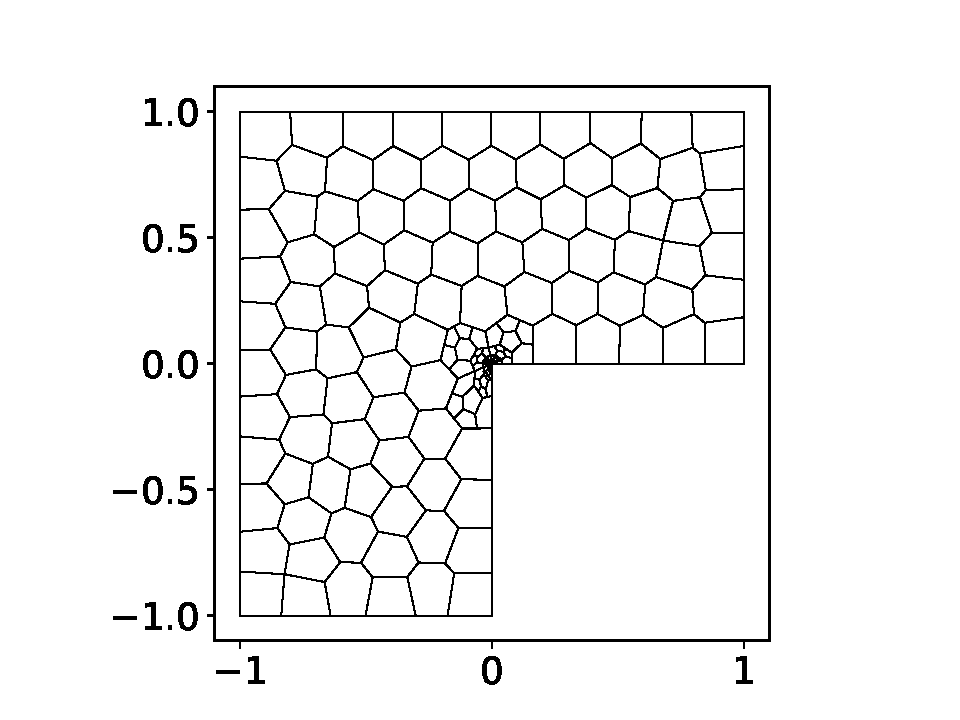
\includegraphics[trim=0cm 0.5cm 0cm 0.5cm, clip, width=5.5cm]{lshape_100_eh1.pdf}
    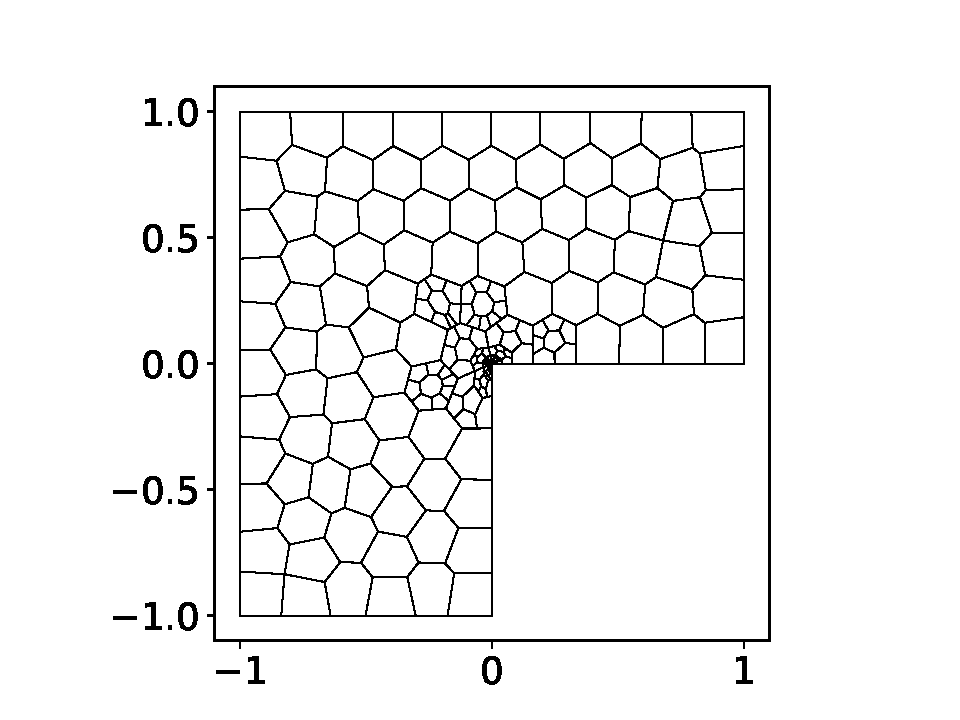
\includegraphics[trim=0cm 0.5cm 0cm 0.5cm, clip, width=5.5cm]{lshape_100_eh2.pdf}
	\caption{L-shaped mesh after 2, 4 and 6 refinements, $N_0 = 100$.}
\end{figure}

\newpage
\subsection{A code snippet}

Here's a snippet to illustrate the mesh size refinement from the user's perspective:

\lstinputlisting[style=cpp, firstline=11]{../snippets/h_refine.cpp}